\chapter{Feature Location Techniques}
\label{ch:feature location techniques}
%\section{Eins - Eins}
%\subsection{Eins - Eins - Eins}

% Die Logos sind veraltet und duerfen zurzeit nicht verwendet werden!
% Auf Seite \pageref{Logo} in Abbildung \ref{Logo} befindet sich das SE Logo.
This chapter deals with five different feature location techniques in detail. They are defined as two static and two dynamic techniques with each one technique giving plain, one giving guided output and the static plain technique \emph{SNAIFL} as a special case. The techniques presented in the following can be classified by the characteristics of \autoref{ch:Classification and Methodology}:

\begin{table}[h]
	\begin{tabular}{|l| l l l l l l|}
		\hline
		 & technique &  output & underlying & input & result & user \\ 
		 &  &  &  technology &  &  &  \\ \hline
		 \multirow{5}{1em}{\begin{sideways} static \end{sideways}}
		 & Find-concept  & plain & PDA, NLP & query & AOIG & ++  \\
		 &      &        &             &         & documents  &   \\
		 & SNIAFL & plain & tf-idf, LSI, & set of query's & BRCG & -/+ \\ 
		 &        &       & PDA  &             &      &
		 \\ 
		 & Dora & guided & PDA, tf-idf & method, depth & call graph & + \\ 
		 &      &        &             & query         & documents  &   \\ \hline
		 \multirow{4}{1em}{\begin{sideways} dynamic \end{sideways}}
		 & Software & plain & FCA, PDA & set of & executable & +++ \\ 
		 & Reconnaissance &  &  & scenarios, query & & \\
		 & Revelle  & guided & trace analysis & scenario and & executable, & +\\
		 &   &  & LSI, HITS & query & documents & \\ \hline
		
	\end{tabular}
	\caption{The techniques discussed further on in this paper}
	\label{table:techniques overview}
\end{table}

In order to define if the technique is suitable for our Freemind Example(\autoref{ch:Freemind Example}) we regard the number of \textit{false-negatives} and \textit{false-positives}. A \textit{false-negative} method is a method stated relevant by the example but is not a relevant feature derived from the technique. A \textit{false-positive} is the opposite.

\section{Static - Plain}
\label{sec:find-concept}
As an example of a static technique with plain output the \emph{Find-concept (short FC)} of David Shepherd, Emily Hill, K. Vijay-Shanker and Lori Pollock of the University of Delaware and also Martin P. Robillard of the McGill University in Canada is a reasonable choice \cite{shepherd2007using}.
The technique makes, as previously mentioned in \autoref{ch:Classification and Methodology}, some assumptions to the underlying code. To apply \emph{FC} the code has to be object-oriented, the comments and identifiers, which are objects and methods, have to be named in a way so that the technique can retrieve domain knowledge. Also it makes the premise that verbs correspond to methods and nouns refer to objects. Also FC defines so called \textit{direct objects}, which are objects corresponding to a verb. In our example the verb $save$ corresponds to $MindMapMapModel$, $MindMapNodeModel$ and $MindMapEdgeModel$, which are therefore the direct objects of $save$.\newline
\emptyLine
The input to the FC is given by the user as a query of description phrases of the feature of interest and after that decomposed into a set of \textit{verb-DO} pairs. In order to improve the result the technique collects related words, like synonyms or verbs in different time forms, and also regards words, which are often mentioned in the context of words from the query. These collected words then get ranked by their similarity to the query words using LSI (\autoref{sec:LSI}), calculating with a variable weight for the synonyms, and the ten most analogous are presented to the user to augment the query with these terms and program methods already matching to the current query.\newline
\emptyLine
The important aspect the user wants to retrieve are the \textit{verb-DO} pairs matching the query. To be able to derive the matching pairs the FC builds an \textit{action-oriented identifier graph model (AOIG)}. The \textit{AOIG} contains four kinds of nodes and two types of edges:
%\vspace{3em} %WARNING: may be shitty

\begin{table}[th]
	\begin{tabular}{r l}
		\textit{verb nodes}: & a node for each specific verb/action \\
		\textit{direct object (DO) nodes}: & a node for each direct object \\
		\textit{verb-DO nodes}: & a node for every \textit{verb-Do} pair. \\
		&(A \textit{DO} can be in multiple \textit{verb-DO} nodes) \\
		\textit{use nodes}: & a node for each incidence of a \textit{verb-DO} pair in comments \\
		& or the source code \\
		 & \\
		\textit{pairing edges}: & connecting every verb and DO to the \textit{verb-DO nodes} \\
		&containing them \\
		\textit{use edges}: & connecting each \textit{verb-DO node} to every corresponding \\
		& \textit{use node}.
	\end{tabular}
\end{table}

After several steps of improving the query the final query traverses through the \textit{AOIG} and filters every \textit{verb-DO} pair containing words of the query, extracting all methods using the filtered pairs and apply \textit{Program Dependency Analysis (PDA)} on it to reveal call relations within the extraction.

Finally the \emph{FC} is able to generate the result graph with methods matching the query as nodes and structural relations between the methods computed by the \textit{PDA}. \cite{shepherd2007using} \newline
Due to the overhead of computing the \textit{verb-DO} pairs out of the query and the step by step improvement of the input the user interaction in Table \ref{table:techniques overview} is rated with "++".

Regarding the Freemind Example of \autoref{ch:Freemind Example} the technique can\footnote{because of the different ways of extending the query the result may differ from others with the same query} result in the following. The input query, which has to be a \textit{verb-DO} pair, equals \textit{(doAutomaticSave, MindMapMapModel)}. Because of the mentioned adding of words, because of similarity or collocating the terms \textit{save} and \textit{saveInternal} may be added to the query. After performing \textit{LSI} (\autoref{sec:LSI}) the result looks like \autoref{graph:Find-Concept - result}.

\begin{figure}
	\centering
	 \begin{tikzpicture}
	\tikzset{vertex/.style = {shape=ellipse,draw,minimum size=3em}}
	\tikzset{edge/.style = {->,> = latex'}}
	% vertices
	\node[vertex] (p1) at  (1,4) {\#1};
	\node[vertex] (p2) at  (5,2) {\#2};
	\node[vertex] (p3) at  (1,2) {\#3};
	\node[vertex] (p4) at  (5,0) {\#4};
	\node[vertex] (p7) at (2,0)  {\#7};
	%edges
	\draw[edge] (p1)  to (p3);
	\draw[edge] (p4)  to (p2);
	\draw[edge] (p7)  to (p3);
	\draw[edge] (p7)  to (p4);
	\end{tikzpicture}
	\caption{The result graph of the \textit{Find-Concept}}
	\label{graph:Find-Concept - result}
\end{figure}
The result fits the real relevant features, as mentioned in \autoref{ch:Freemind Example}, quite well by stating every relevant method as relevant and only stating \#7 as a\textit{false-positive} . The technique fits the example quite well because of the applicable assumptions towards the underlying code, like the object-oriented structure or the verb-object writing distinction.

\section{Static - Guided}
\label{sec:Dora}
The technique presented by \emph{Emily Hill, Lori Pollock} and \emph{K. Vijay-Shanker}, professors of the \textit{University of Delaware} in  \textit{Computer and Information Science}, is named \emph{Dora the Program Explorer} (short: \emph{Dora}})\footnote{Dora comes from exploradora, the Spanish word for a female explorer\cite{hill2007exploring}. Also the name chosen in account of the children's series "\textit{Dora the Explorer}" }\cite{hill2007exploring}.
Dora also uses a call graph $G=(V,E)$ to derive dependency, like the \emph{Find-concept} in \autoref{sec:find-concept}, but combines it with the \emph{tf-idf} ranking method explained in \autoref{sec:tf-idf} with the methods as nodes $n \in V$, it's body as the documents $d(n)$ and edges $e=(n,m) \in E$ if method $n$ calls method $m$. \newline
As an input the user has to yield an initial query, a so called \textit{seed method} $ n_0 \in V$ the examination should start from, and a depth defining a graph-neighbourhood, which should be included in the search(i.e. a maximal distance). \newline
Given the input, Dora proceeds by traversing through the call graph $G$ calculating how suitable the document $d(n)$ of the current node $n$ is by combining the succeeding three values:
\begin{enumerate}
	\item the \emph{tf-idf} score of the identifiers within the method name ($n$)
	\item the \emph{tf-idf} score of the identifiers within the method body ($d(n)$)
	\item a binary value to indicate if the method belongs to a library or is part of the user-made code
\end{enumerate}
Dora can be parametrized by the weight of these three components, for example the method name(1) should be more important than the method body(2) and if the method is out of a library it should not be considered, which leads to the following formula:
\begin{center}
	$\quad s(n)= (1-b) * [ \frac{2}{3} $\emph{tf-idf}$(n) + \frac{1}{3}$\emph{tf-idf}$(d(n)) ]$
\end{center} 
where $b$ defines if $n$ belongs to a library($b=1$) or $n$ is user-made($b=0$).
There are two more adjustable values: the relevance threshold($rt$) and exploration threshold($et$). The relevance threshold determine whether a node is relevant or not can be parametrized by giving a value $rt,et \in [0,1] $ and typically $et < rt$, that given a node $n$:
\vspace{2em} %WARNING: might be shitty
\begin{table}[h]
	\centering
	\begin{tabular}{r c l}
		$rt <= s(n)$ & $\rightarrow$ & the node is relevant\\
		$et <= s(n) < rt$ & $\rightarrow$ & the node is not relevant, but maybe it's neighbours \\
		$s(n) < et$ & $\rightarrow$ & the node can be neglected
	\end{tabular}
\end{table}

In the case of 1 and 2 Dora traverses to the neighbourhood of the node, if it does not harm the initial depth, and otherwise discards the node. So in finite steps of traversing through the call graph Dora has reached a point, where no additional elements need to be explored.\newline
The result Dora computes is a subgraph $G'=(V',E')$ of the call graph, where $V' = \{ n \in V | et <= s(n) \}$, $E' = \{ (n,m) \in E | n,m \in V' \}$ and a function \newline
\[
	f: n\in V' \rightarrow \{0,1\},n \rightarrow 
		\left\{
			\begin{array}{ll} 
				1, & s(n) >= rt \\
				0, & else 
			\end{array}\right. .
\]
This function can be described as a colouring of every \textit{relevant} node. The final output is the coloured sub-call-graph $G'$. \newline
\emptyLine
In the \textit{Freemind Example} of \autoref{ch:Freemind Example} the result can look different, by changing the parameters like the \textit{seed method}, the \textit{depth} or the \textit{threshold values}.
\newline
Simplifying the method in the fact of disregarding the method body's and by knowing that every method called in \autoref{pic:freemind callgraph} is user made, the scores are equal to their score in \autoref{table:tfidf_table}. \newline
The threshold are chosen like the following:
\begin{table}[h]
	\centering
	\begin{tabular}{r l}
		$rt = 0.5$ & methods with a score of 0.5 or higher are considered relevant \\
		$et = 0.1$ & methods with a score of 0.1 or higher should be explored further
	\end{tabular}
\end{table}

So the final graph Dora computes looks like the \autoref{graph:Dora - result} with \#1 being the \textit{seed method}. The green nodes are relevant to the feature, the grey nodes are explored but not relevant. The red node(\#2) is highly relevant to the feature with a \emph{tf-idf score} of 1.454, but is not explored due to the missing path from \#1 to \#2 (with a maximum length of 3).
\begin{figure}[h]
	\centering
	\begin{tikzpicture}
		\tikzset{vertex/.style = {shape=ellipse,draw,minimum size=1.5em}}
		\tikzset{edge/.style = {->,> = latex'}}
		% vertices
		\node[vertex, fill=black!30!green] (p1) at  (0,2) {\#1};
		\node[vertex, fill=black!30!red] (p2) at  (3,2) {\#2};
		\node[vertex, fill=gray] (p3) at  (0,0) {\#3};
		\node[vertex, fill=white] (p4) at  (3,0) {\#4};
		\node[vertex, fill=gray] (p5) at (-1,-1)  {\#5};
		\node[vertex, fill=gray] (p6) at (-1,-2.5) {\#6};
		\node[vertex, fill=white] (p7) at (1,-1)  {\#7};
		\node[vertex, fill=white] (p8) at (1,-2.5) {\#8};
		%edges
		\draw[edge] (p1)  to (p3);
		\draw[edge] (p4)  to (p2);
		\draw[edge] (p7)  to (p3);
		\draw[edge] (p3)  to (p5);
		\draw[edge] (p5)  to (p6);
		\draw[edge] (p7)  to (p4);
		\draw[edge] (p8)  to (p4);
		\draw[edge] (p8)  to (p7);
	\end{tikzpicture}
	\caption{The result graph of \textit{Dora}, with \#1 as \textit{seed method}, \textit{depth}=3, rt=0.5 and et=0.1}
	\label{graph:Dora - result}
\end{figure}
So \emph{Dora} is not a very good technique for this example because of \#2,\#3 and \#4 being \textit{false-negatives} and therefore only deriving \#1 as relevant.


 In modern cases of application the \textit{threshold}-values are chosen by a heuristic of other cases and general knowledge of the underlying program. Including the \textit{methods body} (2) and the binary value of the formula the result can be refined by slightly changing the query or the \textit{threshold's}. \newline
\emph{Dora} only needs a query and a \textit{depth} to compute a result, which takes to further interaction, which is marked within the \autoref{table:techniques overview} with only one "+".

\section{Dynamic - Plain}
\label{sec:Wilde}
One of the most important dynamic plain approaches is the very first one of Norman Wilde and Michael Scully known under the term \emph{Software Reconnaissance} \cite{wilde1995software}. \textit{Software Reconnaissance} tries to define a feature $f$ by getting two sets of scenarios $S_f$ and $\overline{S_f}$ as an input and distinguishing between scenarios that invoke the feature of interest $S_f$ and scenarios that do not $\overline{S_f}$. \newline
Regarding the execution traces \textit{Software Reconnaissance} categorizes methods/lines of code $M$\footnote{the degree of fineness is chosen by the user} into four groups:
\begin{table}[h]
	\begin{tabular}{l}
		1. potentially involved  \\
 		\qquad $I_1 = \{ m \in M | \exists s \in S_f$ s.t. $s$ executes $m \}$ \\
 		\qquad get executed by \underline{at least one} scenario of $S_f$\\
		2. indispensably involved  \\
		\qquad $I_2 = \{ m \in M | \forall s \in S_f : s$ executes $m \}$ \\
		\qquad get executed by \underline{every} scenario of $S_f$\\
		3. uniquely involved  \\
		\qquad $I_3 = \{ m \in M | m \in I_1$ and $\forall s\in \overline{S_f} : s$ does \underline{not} execute $m \}$ \\
		\qquad executed by at least one scenario of $S_f$ and by no scenario of any other feature\\
		4. common components  \\
		\qquad $C = \{ m \in M | \forall s \in S_f \cup \overline{S_f}:s$ executes $m \}$ \\
		\qquad used by every scenario (for example a \textit{main}-method)
	\end{tabular}
\end{table} \newline
The result are the first three sets for every feature $f$ that is set in the query and once the list of all \textit{common} components. Different versions of this technique state, that $I_2 \cap C = \emptyset$.\cite{wilde1995software} \newline
\emptyLine
In our example regarding the two features of $f_1 = automaticSaveFile$ and $f_2 = manualSaveFile$ the execution traces are quite similar owed to the fact, that the \textit{automaticSaveFile}-feature is just a not user triggered \textit{internalSave}. Keeping in mind the call graph(\autoref{pic:freemind callgraph}) methods \#3, \#5 and \#6 will be considered as \textit{common} components, because of the fact that the \textit{automatic save} feature relies on the \textit{manual save} feature. Method \#1 will be considered \textit{uniquely involved} to the feature $f_1$. Methods \#2 and \#4 are in the \textit{potentially involved} set, because not every \textit{automatic save} run uses these components. So we get no \textit{false-positive} and that \#2 and \#4 are \textit{false-negatives} is a matter of defining these sets. Which shows that \textit{Software Reconnaissance} is a suitable technique for the Freemind Example.\newline
\emptyLine
This technique already requires voluminous overhead, because of the two sets of scenarios $S_f$ and $\overline{S_f}$ for every feature.


\section{Dynamic - Guided}
\label{sec:Revelle}
The dynamic guided technique by Meghan Revelle, Bogdan Dit and Denys Poshyvanyk, which are professors at the College of William and Mary in Virginia, is based on a chain of other techniques here and further named as the main author:
\begin{center}
	$Revelle \cite{revelle2010using} \rightarrow Liu \cite{liu2007feature} \rightarrow Poshyvanyk \cite{poshyvanyk2007feature} \rightarrow Marcus \cite{marcus2004semantic}$
\end{center}
The very base technique by Marcus is to take a given input query and convert it into a document in vector space using the in \autoref{sec:LSI} mentioned \textit{LSI}. The technique then separates different software elements, for example methods, and creates separate documents using the identifiers and also converting them into vector space. The identifiers are often separated using typical code style, like the connecting of two words using "\underline{ }" or changing from lower to upper case letters. In order to filter the result the search space is partitioned by refining the documents similarity values, so that in step $i+1$ are only the documents of step $i$, which are higher than a given threshold. After that the user decides which documents are relevant to the feature. Once the user decides that no further document is relevant to the feature the algorithm terminates. \cite{marcus2004semantic} \newline
%In addition to \textit{Marcus} \textit{Poshyvanyk} uses FCA \autoref{sec:FCA} to rank the documents after they are ranked on the similarity to the input query. \textit{Poshyvanyk} takes the first $n$ documents and ranks the \emph{uniquely} appearing terms in the documents based on the similarity the term and the corpus-document in a way, that terms, which are similar to terms in the $n$ documents but not in the rest, are ranked higher. On the other hand terms, which are similar to documents not being in the top $n$ documents, are penalized because might have identifiers for not relevant things with relevant names and therefore would distort the result. After ranking the unique terms \textit{Poshyvanyk} selects the top $k$ terms as \textit{attributes} out of the top $n$ documents, which are the \textit{objects}, and apply FCA \autoref{sec:FCA}. So the user gets not only the space vectors of the similarity of the documents, but also gets a visualization of the terms used within. \newline
\textit{Poshyvanyk} uses a combination of \textit{Marcus} \textit{LSI} method and \textit{execution-trace analysis} \footnote{further information on that topic within the \textit{IEEE}-paper \cite{antoniol2006feature}}. To analyse a program it has to be given as an input in an executable form, to determine which methods are called on a scenario, and a set of documents, which can be defined out of a query with \textit{Marcus}. Also the technique needs two sets of scenarios: one that invoke the feature of interest and one that does not. First the technique ranks the documents like within \textit{Marcus}. After that the scenario sets are executed and execution profiles are derived. By that the methods can be ranked by the appearance within the traces of the scenarios that execute the feature versus the appearance within the other scenarios. The final result of a method is a weighted sum of the \textit{LSI}-rank and the \textit{trace}-rank. So the final output is again a ranked list of methods. \cite{poshyvanyk2007feature} \newline
The technique \textit{Liu} is quite similar to \textit{Poshyvanyk}, with the difference, that instead of using two sets of scenarios \textit{Liu} only works with a single scenario executing the feature of interest. This reduces the overhead of input and also accelerates the process, accepting the fact that the result may not be as accurate as it would be with \textit{Poshyvanyk}. \cite{liu2007feature} \newline
The technique \textit{Revelle} combines \textit{Information Retrieval}, \textit{dynamic} and \textit{web-mining} analysis in order to improve the results of the previous methods. Like \textit{Liu} \textit{Revelle} gets a single scenario that exercises the feature of interest and a query as input. While running the scenario the call graph from the execution trace is constructed, which nodes are methods that are actually executed. Every node gets a score using a web-mining algorithm like the HITS-algorithm mentioned in \autoref{sec:HITS}. After assigning the values \textit{Revelle} filters one of the following two out:
\begin{itemize}
	\item low-ranked methods 
	\begin{itemize}
		\item typically used on \textit{HITS authority score}
		\item methods that are not called often are not extremely important
	\end{itemize}
	\item high-ranked methods 
	\begin{itemize}
		\item typically used on \textit{HITS hub score}
		\item  methods that call very many other methods are not meaningful
	\end{itemize}
\end{itemize} 
The remaining set of methods get ranked by using \textit{Liu} and the final ranked list is returned to the user.
The overall user interaction is quite sparely, because of one scenario and a query about the feature of interest have to be given as an input and therefore rated with "+" in \autoref{table:techniques overview}. \cite{revelle2010using}


In the Freemind Example (\autoref{ch:Freemind Example}) and given a scenario, where the \textit{automaticSaveFile}-feature is executed the methods \#1,\#3, \#5 and \#6 are invoked. Scoring these using the \textit{HITS-Algorithm} of \autoref{sec:HITS} the elements receive their score in \autoref{graph:HITS - after 100 iterations}. Assuming the \textit{HITS-Algorithm} has a significant threshold \#1 will be filtered, because it's authority score of 0. \newline
The remaining methods \#3, \#5 and \#6 are ranked by their \textit{LSI}(\autoref{sec:LSI}) score, which are presented in \autoref{table:lsi-values} with respect to the query \textit{automaticSaveFile}.\newline
The result has regarding our example two \textit{false-positives} (\#5 and \#6) and three \textit{false-negatives} (\#1, \#2 and \#4), which makes it a technique that should not be used for the Freemind Example.


\section{Future Technique Approaches}
\label{sec:SNIAFL}
All of the presented techniques are still under research to improve the results accuracy, the runtime and the amount of user interaction. Even if the last point is not that important in the beginning it can be the most essential due to the possibility of high serialisation. Also the generally preferred technique group is the static one, because of the high amount of pre-computing used to derive scenarios and checking if they invoke the feature and the execution time used to run these.\newline
\textit{W. Zhao, L. Zhang, J. Sun and F. Yang} from the University of Peking in cooperation with \textit{L. Yin} of the Rensselaer Polytechnic Institute are working on an approach of a \textit{static non-interactive} technique by using \textit{Program Dependency Analysis} and \textit{Information Retrieval} technologies \cite{zhao2006sniafl}.\newline
They define two types of functions of a feature:
\begin{enumerate}
	\item \textit{specific functions}:
	functions only used to implement the feature and not used by any other feature.
	\item \textit{relevant functions}:
	functions involved in the implementation of the feature
\end{enumerate}
The set of \textit{specific features} is indisputable a subset of the set of \textit{ relevant features}.
The presentation of the program within the technique is realized with a so called \textit{Branch-Reserving Call Graph (BRCG)}, which is a normal call graph expanded with branching and sequential information. These informations can be used to construct pseudo execution traces for a feature. The \textit{BRCG} can be written as $G=(V,E)$ with the nodes $V$ as a function, a branch or a return statement. Loops are defined as two branch statements: one going through the loop body and one exiting immediately.


\noindent\begin{minipage}{.35\textwidth}
	\vspace{7em}
	\lstset{language=Java}
	\lstinputlisting[
		label=lst:code,
		caption=An example code for BRCG] {src/listings/BRCG-examplecode.java}
\end{minipage}\hfill
\begin{minipage}{.55\textwidth}
	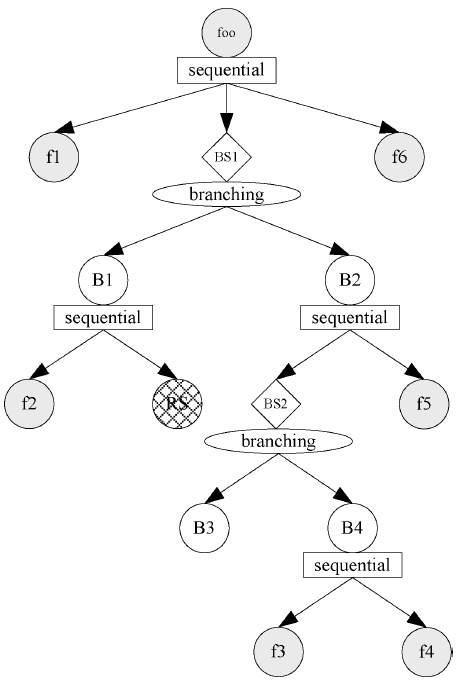
\includegraphics[width=.75\textwidth]{src/pic/BRCG-example.png}
	\captionof{figure}{The BRCG of the example code in \autoref{lst:code} \cite{zhao2006sniafl}}
	\label{graph:BRCG}
	\vspace{2em}
\end{minipage}

In \autoref{graph:BRCG} is shown an example graph for the example code of \autoref{lst:code}, with $f1$ to $f6$ being functions. The nodes $func, B1, B2$ and $B4$ are \textit{sequential} of code, which indicate a sequence of other nodes following, while $BS1$ and $BS2$ are \textit{branching} nodes indicating a conditional-based decision, like an if-statement or a \textit{while}-loop. $RS$ is a \textit{return}-statement and $B3$ is the automatic \textit{exit}-statement previously mentioned.\newline
As an input the technique takes textual paragraphs for every feature, which can be derived by the requirements documentation. These paragraphs are converted into documents using the code style  like in \autoref{sec:Wilde} and normalizing\footnote{in general converting to lower case alphabetical letters} the terms. Also \textit{FCA} (\autoref{sec:FCA}) will be used to convert the methods into queries. \newline
After deriving the documents and queries the technique uses a special \textit{LSI} variation to convert these two sets to a vector space and measure the similarity using the $cosine$. The speciality of this variation is, that the weights of the terms, defining which terms are more important than others, are not given by the user or chosen equally balanced, but are also computed using \textit{tf-idf} (\autoref{sec:tf-idf}).\newline
After these steps the technique has a ranked list $L_d$ of queries(functions) for every document $d$ (feature) ranked by their similarity. Within every list is a pair of queries $p$ with the largest difference so $p^d = max\{ (q^d_i, q^d_{(i+1)}) \in L_d | p^d_i - p^d_{(i+1)} \}$, called \textit{division point}. Every function before the \textit{division point} are considered \textit{initial specific functions} to the feature. \newline
The next step is to traverse the \textit{BRCG} and cut off every branch that does not contain any of the \textit{initial specific functions}, considered to be not relevant to the feature. Vice versa every other function is marked as relevant. So a pseudo-execution can be given to the user as a traversing through the trimmed \textit{BRCG}.\newline

Overall the technique is based on a high amount of computation but works without a single input. \textbf{But} in reality the requirements documentation and comments are not enough to generate that much knowledge about the features, that they can be derived satisfyingly. So the technique works on programs that are written in a certain way, which is not the final solution but is an approach leading the way.




%\clearpage
